% chktex-file 46
\documentclass[12pt]{scrartcl}

\PassOptionsToPackage{utf8}{inputenc}
\usepackage{inputenc}
\usepackage[american]{babel}
\usepackage{csquotes}
\usepackage{microtype}

\usepackage{graphicx}
\graphicspath{{gfx/}}

\usepackage{paralist}
\usepackage{csquotes}
\usepackage[T1]{fontenc}
\usepackage{lmodern}

\usepackage{geometry}
% \geometry{a4paper,body={5.8in,9in}}
\geometry{a4paper}
\renewcommand{\baselinestretch}{1.1}
\usepackage{parskip}
\setlength{\parindent}{0pt}

\usepackage{amsmath, amsfonts, amssymb}
\usepackage{bm}
\usepackage{placeins}
\usepackage{subcaption}

\usepackage{setspace}

\usepackage{hyperref}
\usepackage[nameinlink]{cleveref}
\newcommand{\crefrangeconjunction}{--}

\usepackage[						% use biblatex for bibliography
	backend=bibtex,					% 	- use biber backend (bibtex replacement) or bibtex
	style=numeric,					% 	- use alphabetic (or numeric) bib style
	natbib=true,					% 	- allow natbib commands
	hyperref=true,					% 	- activate hyperref support
	backref=true,					% 	- activate backrefs
	isbn=false,						% 	- don't show isbn tags
	url=false,						% 	- don't show url tags
	doi=false,						% 	- don't show doi tags
	urldate=long,					% 	- display type for dates
	maxnames=3,%
	minnames=1,%
	maxbibnames=5,%
	minbibnames=3,%
	maxcitenames=2,%
	mincitenames=1,%
	sorting=none
]{biblatex}
\bibliography{literature}

\usepackage[inline]{enumitem}
\usepackage{todonotes}
\usepackage{pgfgantt}

% Colors:
\definecolor{blau}{HTML}{355FB3}
\definecolor{rot}{HTML}{B33535}
\definecolor{gruen}{HTML}{3BB335}
\definecolor{hellblau}{HTML}{8ea7d7}
\definecolor{hellgrau}{HTML}{cccccc}

%%%%%%%%%%%%%%%%%%%%%%%%%%%%%%%%%%%%%%

\newcommand{\thesisTitle}{Learning to Aggregate on Structured Data}
\newcommand{\thesisSubject}{Master Thesis Proposal \& Work Plan}
\newcommand{\thesisName}{Clemens Damke}
\newcommand{\thesisMail}{cdamke@mail.uni-paderborn.de}
\newcommand{\thesisMatNr}{7011488}
\hypersetup{% setup the hyperref-package options
    pdftitle={\thesisTitle},    %   - title (PDF meta)
    pdfsubject={\thesisSubject},%   - subject (PDF meta)
    pdfauthor={\thesisName},    %   - author (PDF meta)
    plainpages=false,           %   -
    colorlinks=false,           %   - colorize links?
    pdfborder={0 0 0},          %   -
    breaklinks=true,            %   - allow line break inside links
    bookmarksnumbered=true,     %
    bookmarksopen=true          %
}

\begin{document}

\title{\thesisTitle}
\subtitle{\thesisSubject}
\author{{\thesisName}\\\small{Matriculation Number: \thesisMatNr}\\\small{\href{mailto:\thesisMail}{\thesisMail}}}
\date{\today}
\maketitle

\section{Motivation}%
\label{sec:motivation}

Most of the commonly used supervised machine learning techniques assume that instances are represented by $d$-dimensional feature vectors $x_i \in \mathcal{X} = \mathcal{X}_1 \times \cdots \times \mathcal{X}_d$ for which some target value $y_i \in \mathcal{Y}$ should be predicted.
In the regression setting the target domain $\mathcal{Y}$ is continuous, typically $\mathcal{Y} = \mathbb{R}$, whereas $\mathcal{Y}$ is some discrete set of classes in the classification setting.

Since not all data is well-suited for a fixed-dimensional vector representation, approaches that directly consider the structure of the input data might be more appropriate in such cases.
One such case is the class of so-called \textit{learning to aggregate} (LTA) problems as described by \citet{Melnikov2016}.
There the instances are represented by compositions $\bm{c}_i$ of constituents $c_{i,j} \in \bm{c}_i$, i.e.\@ variable-size multisets with $n_i = |\bm{c}_i|$.
The assumption in LTA problems is that for all constituents $c_{i,j}$ a local score $y_{i,j} \in \mathcal{Y}$ is either given or computable.
The set of those local scores should be indicative of the overall score $y_i \in \mathcal{Y}$ of the composition $\bm{c}_i$.
LTA problems typically require two subproblems to be solved:
\begin{enumerate}[label=\textbf{\arabic*.}]
	\item \textbf{Aggregation:}
		A variadic aggregation function $A: \mathcal{Y}^{*} \to \mathcal{Y}$ that estimates composite scores has to be learned, i.e.\@ $y_i \approx \hat{y}_i = A(y_{i,1}, \dots, y_{i,n_i})$.
		Typically the aggregation function $A$ should be associative and commutative to fit with the multiset-structure of compositions.
	\item \textbf{Disaggregation:}
		In case the constituent scores $y_{i,j}$ are not given, they have to be derived from a constituent representation, e.g.\ a vector $v_{i,j} \in \mathcal{V}$.
		To learn this derivation function $f: \mathcal{V} \to \mathcal{Y}$, only the constituent vectors ${\{v_{i,j}\}}_{j = 1}^{n_i}$ and the composite score $y_i$ is given.
		Thus the constituent scores $y_{i,j}$ need to be \textit{disaggregated} from $y_i$ in order to learn $f$.
\end{enumerate}
Overall LTA can be understood as the joint problem of learning the aggregation function $A$ and the local score derivation function $f$.

Current LTA approaches only work with multiset inputs.
In practice there is however often some relational structure among the constituents of a composition.
This effectively turns LTA into a graph regression problem.
The goal of this thesis is to look into the question of how aggregation function learning methods might be generalized to the graph setting.

\section{Related Work}%
\label{sec:related-work}

This thesis will be based on two currently mostly separate fields of research:
\begin{enumerate*}[label=\textbf{\arabic*.}]
	\item Learning to Aggregate
	\item Graph classification \& regression
\end{enumerate*}.
A short overview of the current state-of-the-art approaches in both fields will be given now.

\subsection{Learning to Aggregate}%
\label{sec:related-work:lta}

Two main approaches to represent the aggregation function in LTA problems have been explored.
The first approach uses \textit{uninorms}~\cite{Melnikov2016} to do so.
There the basic idea is to express composite scores as fuzzy truth assignments $y_i \in [0, 1]$.
Such a composite assignment $y_i$ is modeled as the result of a parameterized logical expression of constituent assignments $y_{i,j} \in [0, 1]$.
As the logical expression that thus effectively aggregates the constituents, a uninorm $U_{\lambda}$ is used.
Depending on the parameter $\lambda$, $U_{\lambda}$ combines t-norms and t-conorms which are continuous generalizations of logical conjunction and disjunction respectively.

Recently \citet{Melnikov2019} have also looked at an alternative class of aggregation functions.
Instead of using fuzzy logic to describe score aggregation, \textit{ordered weighted average} (OWA) operators were used.
OWA aggregators work by sorting the input scores and then weighting them based on their sort position, i.e.\ %
\begin{align*}
	A_{\lambda}(y_1, \dots, y_n) := \sum_{i = 1}^n \lambda_i y_{\pi(i)},
\end{align*}
where $\lambda$ is a weight vector with ${\|\lambda\|}_1 = 1$ and $\pi$ is a sorting permutation of the input scores. % chktex 21
To deal with varying composite sizes $n$ the weights $\lambda_i$ are interpolated using a \textit{basic unit interval monotone} (BUM) function $q: [0, 1] \to [0, 1]$.
It takes constituent positions that are normalized to the unit interval, i.e.\ $\frac{i}{n}$.
The BUM function $q$ then is then used to interpolate a weight for any normalized sort position via $\lambda_i = q(\frac{i}{n}) - q(\frac{i - 1}{n})$.
Therefore the learning objective boils down to optimizing the shape of $q$.
The details of this are left out here.

\subsection{Graph Classification and Regression}%
\label{sec:related-work:gcr}

As previously mentioned, the addition of relations between constituents turns LTA into a graph regression problem.
Most of the recent research in the field of learning from graph structured data has however focused on the closely related graph classification problem.
Since many ideas from the classification setting are also useful in the regression setting, a brief overview of those ideas is given first.

At a high level graph classification methods can be taxonomized into two main families:
\begin{enumerate}[label=\textbf{\arabic*.}]
	\item \textbf{Vector representation approaches:}
		One way to tackle the graph classification problem is to map an input graph $G$ to a vectorial representation.
		This can be done
		\begin{enumerate*}
			\item by either handpicking global graph features like vertex/edge count, degree distribution or graph diameter,
			\item via a graph embedding algorithm like node2vec~\cite{Grover2016}, sub2vec~\cite{Adhikari2018} or graph2vec~\cite{Narayanan2017},
			\item implicitly by using a graph kernel that computes the structural similarity between graphs, e.g.\ the Weisfeiler-Lehman kernel~\cite{Shervashidze2011} or the multiscale Laplacian graph kernel~\cite{Kondor2016}
		\end{enumerate*}.
		Graphs can then be classified via any classification algorithm that works with vectors and/or kernels.
	\item \textbf{Graph neural networks:}
		An alternative approach is to adapt neural networks to graph inputs.
		The notion of a \textit{graph neural network} (GNN) was first introduced by \citet{Gori2005}.\@
		There a message-passing architecture is used to iteratively propagate vertex information to neighbors until a fixed point is reached.
		This process is computationally expensive.

		Recently the class of \textit{convolutional graph neural networks} (ConvGNNs) gained traction.
		It generalizes the convolution operator that is used by \textit{convolutional neural networks} (CNNs) to graphs.
		There are two main variants of ConvGNNs:
		\begin{enumerate}[label=\textbf{\alph*)}] % chktex 9 chktex 10
			\item \textbf{Spatial variant:}
				Standard CNNs use a convolution operator that is typically applied to a grid graph of pixels with added diagonal edges.
				Spatial ConvGNNs~\cite{Micheli2009} directly generalize this idea by defining a more flexible convolution that works with arbitrary graph structures.
				Spatial graph convolution aggregates the direct neighborhood of a vertex $v_i$, where $v_i$ is typically described by a feature vector $x_i \in \mathbb{R}^d$.
				This process returns a new aggregate feature vector $x'_i$.
				By stacking multiple convolution layers, features from indirect neighbors become part of the aggregate.
				Analogous to how CNNs learn kernel matrices, spatial ConvGNNs learn vertex neighborhood feature aggregation functions.
				This approach shares similarities with the previously mentioned message-passing architecture~\cite{Gori2005} with the major different being that the number of message-passing, i.e.\ convolution, steps is fixed.
			\item \textbf{Spectral variant:}
				Motivated by the theoretical foundation provided by spectral graph theory~\cite{Shuman2013}, spectral ConvGNNs~\cite{Bruna2013} learn a filter function $\hat{g}$ that is applied in the Fourier domain of a graph.
				Based on the convolutional theorem, a convolution operator can not only be expressed in terms of the neighborhood of vertices but also as a filter on the eigenvectors of a graph's Laplacian.
				Formally this can be expressed as
				\begin{align}
					g *_G \bm{x} = U \hat{g}(\Lambda) U^{\top} \bm{x}\label{eq:related-work:conv-filter}
				\end{align}
				where $\bm{x} \in \mathbb{R}^{n \times k}$ is the matrix of all vertex features and $U \Lambda U^{\top}$ is the eigendecomposition of the graph Laplacian $L_G$\footnote{
					To see the connection to the convolutional theorem, note that $\mathcal{F} = U$ and $\mathcal{F}^{-1} = U^{\top}$ in \cref{eq:related-work:conv-filter} with $\mathcal{F}$ denoting the graph Fourier transform.
				}.
				In the previously described spatial ConvGNN variant, $g$ is learned directly in form of the feature aggregation function with a neighborhood locality constraint.
				In the spectral variant however the Fourier-transformed filter $\hat{g}$ is learned.
				Intuitively this means that vertex features $x_i$ are not aggregated with the features of their their direct neighborhood but with the features of vertices with which they share certain structural similarities.
				This allows spectral ConvGNNs to incorporate the global graph structure at the cost of having to perform the computationally expensive decomposition of every input graph's Laplacian.

				To tackle the performance impact of the spectral convolution approach, various simplifications of the filter $\hat{g}$ have been proposed.
				The so-called \textit{graph convolutional network}~(GCN)~\cite{Kipf2017} does this by reducing the expressivity of the filter.
				Then $\hat{g}$ can be applied to the Laplacian directly via $g *_G \bm{x} = \hat{g}(L_G) \bm{x}$ which saves the decomposition costs.
				This simplification of $\hat{g}$ implicitly causes its Fourier inverse $g$ to be locality constrained just like in the spatial ConvGNN variant.
				Hence the spectral GCN approach also allows for a spatial/message-passing interpretation.
				Recently various variants and extensions of GCNs~\cite{Hamilton2017}\cite{Chen2018}\cite{Chen2017}\cite{Chiang2019}\cite{Du2017} have been proposed that apply additional approximations and sampling methods to improve the runtime as well as the accuracy in certain scenarios.

				One notable extension of GCNs are the so-called \textit{adadptive graph convolutional networks} (AGCNs)~\cite{Li2018}.
				AGCNs do not use a fixed Laplacian $L$ for each input but instead learn a so-called residual Laplacian $L_\mathit{res}$.
				The residual Laplacian is constructed by learning a vertex similarity kernel $\mathbb{G}_{x_i,x_j}$ which is used to determine edge weights between vertices.
				By overlaying the learned residual Laplacian $L_\mathit{res}$ on top of the given intrinsic Laplacian $L$, similar nodes with a large spatial distance in $L$ become connected.
				This can improve the accuracy especially if a locality constrained spectral filter $\hat{g}$ is used.
		\end{enumerate}

		The just described ConvGNN approaches generally assume that an input consists of an undirected graph with positive real edge weights.
		Those approaches are not directly applicable in scenarios with multiple edge types, i.e.\ multi-relational scenarios.
		One class of spatial multi-relational GNN methods was proposed by \citet{Battaglia2018}.
		They describe a general framework for the construction of GNNs; for simplicity only the class message-passing variants is mentioned here.
		There a shared function $\phi^e$ is used to describe how a vertex feature vector $v_i$ is transformed as it passes through an edge with features $e_{ij} \in \mathbb{R}^p$.
		In a uni-relational spatial GNN with $e_{ij} \in \mathbb{R}^{1}$, typically $\phi^e(e_{ij}, v_i) = e_k \cdot v_i$ is used.
		In the multi-relational setting, $\phi^e$ can instead be learned via a standard \textit{multilayer perceptron} (MLP).
		An alternative spectral multi-relational ConvGNN approach was proposed by \citet{Gong2018}.
		Their so-called \textit{edge enhanced graph neural network} (EGNN) essentially models each relation as a separate graph with its own Laplacian.
		A convolutional filter $g$ is shared across all relations and used to convolve the input signal separately via each relation's Laplacian.
		To share vertex features across relations, the separately convolved signals of all relations are then concatenated.
		Those concatenated vertex features are used as the input signal of the next layer.

		This concludes the short overview of approaches to learn vertex feature vectors via ConvGNNs.
		After the application of either spatial or spectral graph convolutions, each vertex will have an updated aggregate feature vector.
		To obtain an aggregate score for the entire graph, a graph pooling layer is applied.
		A primitive pooling approach is to simply merge the vertex features via a fixed aggregation function like $\min$, $\max$ or $\text{avg}$.
		Better results can be obtained by learning the pooling aggregation function.
		Two notable graph pooling approaches are \textit{SortPooling}~\cite{Zhang2018} and \textit{Self-Attention Pooling}~\cite{Lee2019}.
		\begin{enumerate}
			\item SortPooling assumes that the vertex feature vectors are obtained using a stack of spectral convolution layers that learn filters on the random walk Laplacian $L = I - D^{-1} A$.
				This assumption makes it possible to interpret the outputs of the graph convolution layers as a continuous generalization of \textit{Weisfeiler-Lehman} (WL) colors.
				WL colors are lexicographically sortable signatures that encode the structural role of vertices; they can be used for efficient graph isomorphism falsification~\cite{Weisfeiler1968}.
				Using this interpretation of the vertex feature vectors, SortPooling determines a top-$k$ ranking of the vertices' WL colors and then aggregates the thus selected fixed-size vertex feature subset via a MLP.\@
			\item Self-Attention Pooling adds an additional graph convolution layer after an arbitrary ConvGNN.\@
				The added layer takes the aggregated vertex feature vectors as input and outputs a score for each vertex.
				This score is used to determine a top-$k$ vertex ranking.
				Unlike SortPooling the feature vectors of the resulting subset are first added up.
				The resulting aggregate graph feature vector is then fed into a MLP to obtain a class.
		\end{enumerate}
\end{enumerate}

While all of the previously mentioned problems were evaluated on graph classification problems, they can naturally be extended to regression tasks.
In the case of ConvGNNs for example, the described pooling layers already produce continuous outputs.

The pooling aggregation functions used in ConvGNNs are however typically not part of the learning objective.
This shows the fundamental methodological difference between GNNs and LTA.\@
A GNN uses the relational structure of its input to try to determine meaningful feature representations or scores for each vertex.
Those vertex scores are then combined using a simple aggregation function.
LTA on the other hand currently does not use any relational structure and therefore computes vertex/constituent scores independently.
Those comparatively less meaningful local scores are then combined using a more expressive learned aggregation function.
Generally speaking current GNN approaches focus on the disaggregation problem while LTA approaches focus on the aggregation problem.
The described Self-Attention Pooling~\cite{Lee2019} can be seen as an exception to this generalization since it learns an aggregation function in form of the self-attention vertex weights.

\subsection{Molecular Analysis Problems and Datasets}%
\label{sec:related-work:tox}

Graph regression problems have for the most part only been discussed in the context of specific domain problems.
One of those domains is the prediction of chemical toxicity, typically the $\text{LD}_{50}$ or $\text{LC}_{50}$ doses which measure the smallest amount of a given chemical that is lethal for at least $50\%$ of tested subjects.
Another regression task from the domain of molecular analysis is the prediction of compound solubility.
The following approaches could serve as inspiration, baselines and/or sources of training data:
\begin{itemize}
	\item \textit{RASAR}~\cite{Luechtefeld2018} uses a logistic regression model.
		It is trained with manually chosen features that are given for training molecule graphs.
		To predict the toxicity of a new chemical, $k$-means is used to average the features of chemicals with similar molecule graphs in the training set.
		The structural similarity between molecule graphs is measured by the Tanimoto coefficient of their chemical fingerprints.
		Those fingerprints encode the presence or absence of certain meaningful chemical substructures.
		The implementation and used dataset is unfortunately not publicly available because it is part of a commercial product\footnote{ToxTrack Inc., \url{https://toxtrack.com/}}.
	\item \textit{ProTox}~\cite{Drwal2014}\cite{Banerjee2018} is another toxicity prediction approach.
		It works similarly to RASAR but leaves out the logistic regression step and instead directly aggregates the toxicity of similar chemicals via $k$-means.
		ProTox uses the freely available \textit{SuperToxic} dataset~\cite{Schmidt2009} which contains 13400 molecules with known $\text{LD}_{50}$ values.
		While the implementation is again not publicly available, the trained model can be freely queried online\footnote{ProTox-II, \url{http://tox.charite.de/protox_II/}}.
	\item The \textit{Toxicity Estimation Software Tools}~(T.E.S.T.)\footnote{\url{https://www.epa.gov/chemical-research/toxicity-estimation-software-tool-test}} is a free collection of models for toxicity prediction.
		Like RASAR and ProTox it includes similarity-based prediction models but also linear regression and decision tree models that are trained on vector representations of chemicals.
		The publicly available \textit{ChemIDplus}\footnote{\url{https://chem.nlm.nih.gov/chemidplus/}} database was used for training.
		It contains 28023 and 13541 molecules with known oral $\text{LD}_{50}$ values for rats and mice respectively.
		Additionally about 1000 molecules with known $\text{LC}_{50}$ values are available for both species.
	\item Recently first toxicity prediction approaches using ConvGNNs have been published.
		The previously mentioned AGCN~\cite{Li2018} was in fact evaluated on a discrete toxicity classification problem;
		this could serve as a starting point for a continuous graph regression method.
		\citet{Pope2018} describe how functional groups of toxic chemicals can be learned using GCNs;
		there a functional group refers to a relevant subgraph of a molecule that can be interpreted as a toxicity indicator.
	\item The previously described EGNN method~\cite{Gong2018} for multi-relational graphs was evaluated on a compound solubility prediction task.
		For this the Lipophil\-icity~\cite{Wu2017} and FreeSolv~\cite{Mobley2014} datasets were used.
		They contain 4200 and 642 labeled molecular graphs respectively.
\end{itemize}

\section{Research Questions}%
\label{sec:question}

When looking only at the input and output of the described LTA and graph methods, they share certain similarities.
Both take a variable size and permutation invariant set of constituents/vertices as input and compute an aggregate class or score from it.
There is however a difference between LTA and the described graph methods in the way aggregate scores are computed.

LTA approaches are based on the assumption that a composite score can be modeled as an aggregate of constituent scores where constituent and composite scores are required to be from the same domain, e.g.\ $\mathcal{Y} = [0, 1]$.
One consequence of this assumption is that an aggregate score is explainable by looking at the constituents and their associated scores.

A graph classification or regression method on the other hand does not necessarily output explainable classes or scores.
ConvGNNs for example perform multiple neighborhood feature aggregations around each vertex and then combine the aggregated vertex features into a final output using either a fixed aggregation function (e.g.\ $\min$, $\max$ or $\text{avg}$) or a standard predictor that gets a fixed-size top-$k$ ranking of the vertex features.
A given aggregate score is generally not explained by the presence or absence of certain constituents.

Intuitively the difference between LTA and current graph methods can be formulated as \textit{first evaluate, then aggregate} versus \textit{first aggregate, then evaluate}, see \cref{fig:gnnvslta}.
This general difference is however not a strict separator of LTA and current graph methods.
As described by \citet{Pope2018} for example, relevant subgraphs with a high influence on the output of a ConvGNN can be identified and interpreted similarly to LTA constituents.
The line between both approaches is therefore blurry.
\begin{figure}[h]
	\centering
	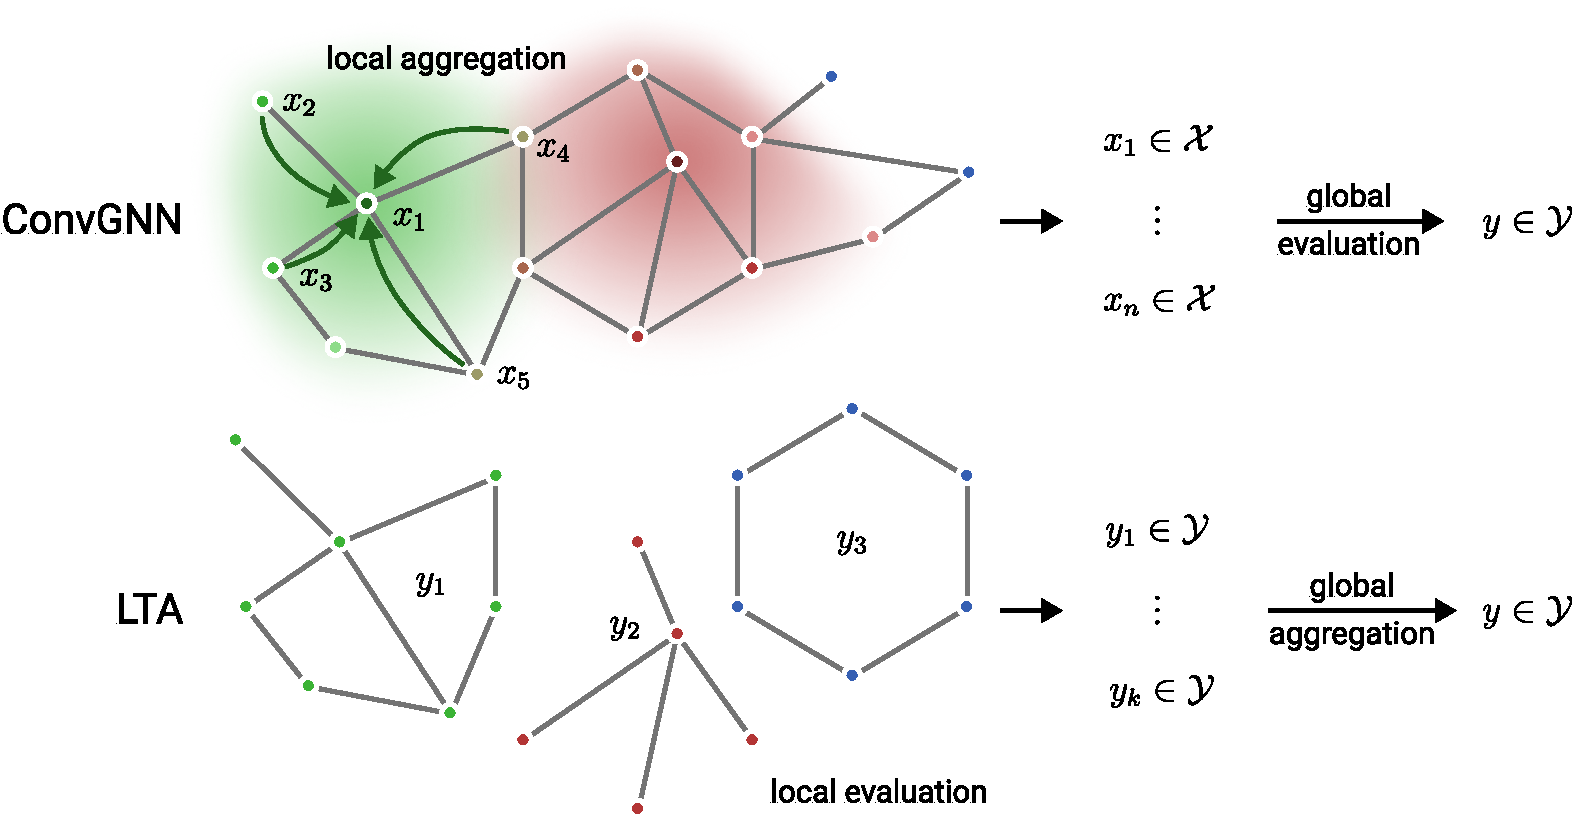
\includegraphics[width=0.9\linewidth]{GNNvsLTA.pdf}
	\caption{Intuition for the difference between ConvGNNs and LTA methods.}\label{fig:gnnvslta}
\end{figure}

To address this, the thesis should try to answer three central questions:
\begin{enumerate}
	\item \textit{What are the essential characteristics of a Learning to Aggregate method?}
		Those characteristics should formally capture the differences and similarities between LTA and convolutional or kernel based graph methods.
		Currently there is no comprehensive formulation of the relation between both fields of research;
		this should be addressed by the first question.
	\item \textit{How could a Learning to Aggregate method, that has the previously defined characteristics, look like for graph inputs?}
		Currently LTA has only been applied to sets of constituents and not yet to graph structured data;
		this should be addressed by the second question.
	\item \textit{What are the assumptions of graph LTA methods and under which circumstances are they applicable?}
		This aims to clarify in which kinds of scenarios the use of LTA is justified and expected to improve results compared to more general methods.
\end{enumerate}

\section{Approach}%
\label{sec:approach}

To answer the three research questions, the following approach will be taken.
First the notion of composites and constituents should be generalized based on the definitions found in the previous works on LTA~\cite{Melnikov2016}\cite{Melnikov2019}, so that they are also applicable to graph inputs.
Next the notion of an aggregation function has to be defined and distinguished from the more general concept of an evaluation function (compare \cref{fig:gnnvslta}).

The resulting general definition of LTA methods should then be used for a comparison with a representative selection of existing graph methods (see \cref{sec:related-work:gcr}).
It should be stated how both fields of research are related and under which circumstances a graph method can be interpreted as an LTA method.
When formulating a graph method from the LTA perspective, it must be explicitly stated how the constituents and the aggregation function looks like.
Depending on the graph method a constituent could consist of a single vertex but could also represent a certain subgraph or characteristic graph pattern.

The comparison between LTA and existing graph methods should serve as an overview of the state-of-the-art in graph classification and regression from the perspective of LTA.\@
Based on this comparison, a specific graph LTA method or class of graph LTA methods should be developed.
Depending on the interpretability of existing graph methods as LTA methods, the developed method will potentially be based on those existing methods.

Finally the proposed graph LTA method should be evaluated.
For this synthetically generated data or some of the datasets listed in \cref{sec:related-work:tox} could be used.
If time permits, a comparison between the developed graph LTA method and other graph methods should be conducted to empirically demonstrate the potential advantages and disadvantages of the LTA assumptions.

\section{Preliminary Document Structure}%
\label{sec:doc-structure}

\begin{enumerate}
	\item Introduction
	\item Previous Work
		\begin{enumerate}[label*=\arabic*.]
			\item Learning to Aggregate
			\item Convolutional Graph Neural Networks
		\end{enumerate}
	\item Learning to Aggregate on Graphs
	\begin{enumerate}[label*=\arabic*.]
		\item Characteristics of LTA methods
		\item An LTA perspective on GNNs
		\item A Graph LTA Method
	\end{enumerate}
	\item Evaluation
	\item Conclusion
	\item Literature
	\item Appendix
\end{enumerate}

\section{Time-Schedule}%
\label{sec:schedule}

\begin{figure}[!ht]
	\centering
	\begin{ganttchart}[
		x unit = 0.55cm,
		y unit title = 0.6cm,
		y unit chart = 0.7cm,
		vgrid,
		canvas/.style = {
			draw = none
		},
		title label font = \sffamily,
		title height = 1,
		title/.style = {
			draw = none,
			fill = none
		},
		group label font = \sffamily\bfseries,
		group label node/.append style = {
			left = 0.2cm
		},
		group/.append style = {
			fill = blau,
			draw = none
		},
		group peaks tip position = 0,
		bar label font = \sffamily\bfseries,
		bar label node/.append style = {
			left = 0.2cm
		},
		bar/.append style = {
			fill = blau,
			draw = none
		}
	]{1}{20}
		\gantttitle{week}{20} \\
		\gantttitlelist{1,...,20}{1} \\ % ignore triple dots: chktex 11

		\ganttgroup{Implementation}{2}{12} \\
		\ganttbar[bar label font = \sffamily, bar/.append style = {fill = hellblau}]
			{Data Preparation}{2}{2} \\
		\ganttbar[bar label font = \sffamily, bar/.append style = {fill = hellblau}]
			{Graph LTA}{3}{8} \\
			\ganttbar[bar label font = \sffamily, bar/.append style = {fill = hellgrau}]
				{Buffer}{9}{10} \\
		\ganttbar[bar label font = \sffamily, bar/.append style = {fill = hellblau}]
			{Evaluation}{11}{12} \\

		\ganttgroup{Writing}{1}{19} \\
		\ganttbar[bar label font = \sffamily, bar/.append style = {fill = hellblau}]
			{Previous Work}{1}{4} \\
		\ganttbar[bar label font = \sffamily, bar/.append style = {fill = hellblau}]
			{Graph LTA}{5}{10} \\
		\ganttbar[bar label font = \sffamily, bar/.append style = {fill = hellblau}]
			{Evaluation}{11}{13} \\
		\ganttbar[bar label font = \sffamily, bar/.append style = {fill = hellblau}]
			{Conclusion}{14}{14} \\
		\ganttbar[bar label font = \sffamily, bar/.append style = {fill = hellgrau}]
			{Buffer}{15}{17} \\
		\ganttbar[bar label font = \sffamily, bar/.append style = {fill = hellblau}]
			{Corrections}{18}{19} \\

		\ganttbar{Presentation}{19}{20}
	\end{ganttchart}
	\caption{Sketch of the time schedule for the work on the thesis}\label{fig:schedule}
\end{figure}

% % %
\newpage
{%
\renewcommand{\bibfont}{\normalfont\small}
\setlength{\biblabelsep}{5pt}
\setlength{\bibitemsep}{0.5\baselineskip plus 0.5\baselineskip} % chktex 1
\setcounter{biburllcpenalty}{9000}
\setcounter{biburlucpenalty}{9999}
\printbibliography%
}

\null\vfill

\begin{center}
	\begin{tabular}{l p{0.1\textwidth} r}
		\cline{1-1} \cline{3-3}
		\begin{minipage}[t]{0.4\textwidth}
			\centering
			\vspace{0cm}Supervisor
		\end{minipage}
		&
		\begin{minipage}[t]{0.2\textwidth}
		\end{minipage}
		&
		\begin{minipage}[t]{0.4\textwidth}
			\centering
			\vspace{0cm}Student
		\end{minipage}
	\end{tabular}
\end{center}

\end{document} % chktex 17
